\subsubsection*{\underline{\textsc{\Large Skeleton}}}
\noindent\emph{Medium undead, neutral evil}

\noindent\rule{0.5\textwidth}{0.5pt}

\noindent\textbf{Armor Class}: 13

\noindent\textbf{Hit Points}: 13 (2d8 + 4)

\noindent\textbf{Speed}: 30 ft.

\noindent\rule{0.5\textwidth}{0.5pt} \\
\begin{table}[H]
	\begin{tabular}{cccccc}
		\textbf{STR} & \textbf{DEX} & \textbf{CON} & \textbf{INT} & \textbf{WIS} & \textbf{CHA} \\
		10 (+0) & 14 (+2) & 15 (+2) & 6 (-2) & 8 (-1) & 5 (-3) \\
	\end{tabular}
\end{table}
\noindent\rule{0.5\textwidth}{0.5pt} \\

\noindent\textbf{Damage Vulnerabilities}: bludgeoning

\noindent\textbf{Damage Immunities}: poison

\noindent\textbf{Condition Immunities}: exhaustion, poisoned

\noindent\textbf{Senses}: darkvision 60 ft., passive Perception 9

\noindent\textbf{Languages}: understands the languages it knew in life but can't speak

\noindent\textbf{Challenge}: 1/4 (50 XP)

\noindent\rule{0.5\textwidth}{0.5pt}

\noindent\textbf{ACTIONS}

\noindent\textbf{Shortsword}: Melee Weapon Attack: +4 to hit, reach 5 ft., one target. Hit: 5 (1d6 + 2) piercing damage.

\noindent\textbf{Shortbow}:  Ranged Weapon Attack: +4 to hit, range 80/320 ft., one target. Hit: 5 (1d6 + 2) piercing damage.

\begin{center}
	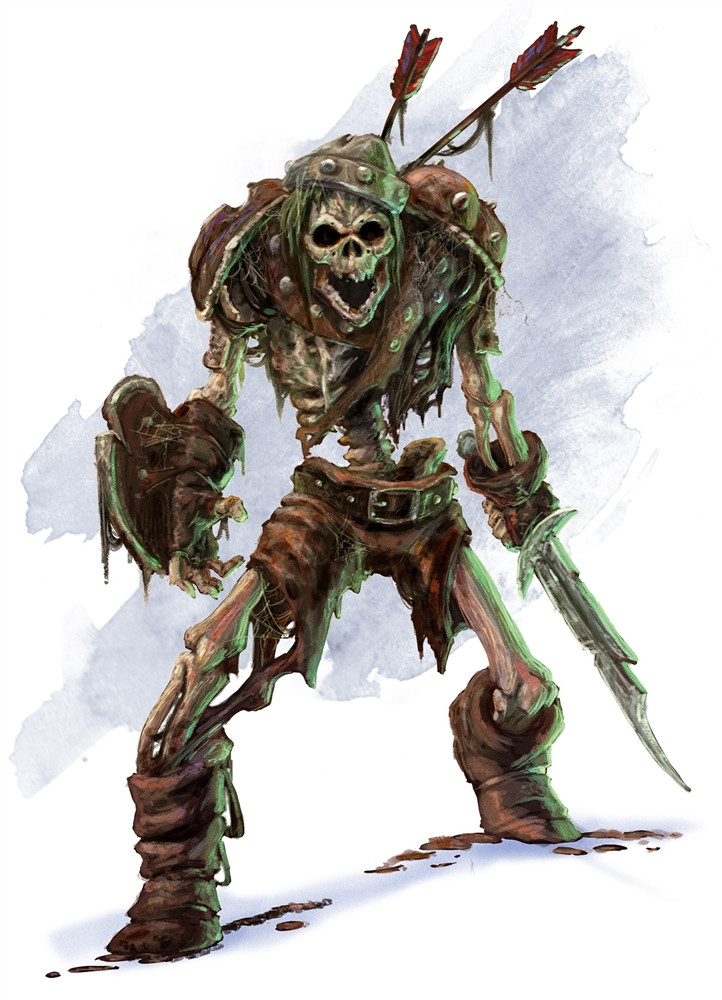
\includegraphics[width = 0.3\textwidth]{skeleton}
	
	\emph{Skeleton}
\end{center}